%% --------------------------------*- Latex -*---------------------------------
%% Filename: master.tex
%% Description: 
%% Author: Fabian Wermelinger
%% Email: fabianw@student.ethz.ch
%% Created: Sat Jul 23 19:36:14 2011 (+0200)
%% Version: 
%% Last-Updated: Thu Dec 15 20:23:19 2011 (+0100)
%%           By: Fabian Wermelinger
%%     Update #: 14
%% ----------------------------------------------------------------------------
%%% master.tex starts here
%% ----------------------------------------------------------------------------

%Preamble
%------------------------------------------------------------------------------
\documentclass[11pt,a4paper]{article}
%% --------------------------------*- Latex -*---------------------------------
%% Filename: header.tex
%% Description: 
%% Author: Fabian Wermelinger
%% Email: fabianw@student.ethz.ch
%% Created: Sat Jul 23 19:33:31 2011 (+0200)
%% Version: 
%% Last-Updated: Thu Dec 15 15:57:37 2011 (+0100)
%%           By: Fabian Wermelinger
%%     Update #: 13
%% ----------------------------------------------------------------------------
%%% header.tex starts here
%% ----------------------------------------------------------------------------

%Macros
%------------------------------------------------------------------------------
\usepackage[utf8x]{inputenc}
%\usepackage[]{ngerman}
\usepackage[english]{babel}
\usepackage[T1]{fontenc}
\usepackage[]{a4}
\usepackage[text={15cm,23.5cm},centering]{geometry}
\usepackage[]{amsmath, amssymb, amsthm, amsfonts}
\usepackage[]{mathrsfs}
\usepackage[]{bm}
\usepackage[]{latexsym}
\usepackage[font=small,labelfont={bf,sf},labelsep=quad,%
figurename=Figure,tablename=Table,margin=20pt]{caption}
\usepackage[]{cite}
\usepackage[]{fancyhdr}
%\usepackage[section]{placeins}
\usepackage[pdftex]{graphicx}
%\usepackage[]{pstricks, pst-all, pst-3dplot}
\usepackage[]{xcolor}
\usepackage[]{psfrag}
\usepackage[]{afterpage}
\usepackage[]{fancyvrb}
\usepackage[]{float}
\usepackage[]{subfig}
\usepackage[]{xspace}
\usepackage[]{nomencl}
\usepackage[]{url}
\usepackage[]{calc}
\usepackage[]{multirow}
\usepackage[]{slashbox, pict2e}
\usepackage[]{setspace}
\usepackage[]{appendix}
%\usepackage[sf]{titlesec}
%\usepackage[scaled=0.93]{helvet}
%\usepackage[]{mathpazo}
%\usepackage[]{layouts}
%\newcommand\showpage{%
%\currentpage\pagedesign}
%\usepackage{program}
\usepackage{algorithmic}

%Text layout
%------------------------------------------------------------------------------
\setlength{\unitlength}{1cm}
\setlength{\topmargin}{-1cm}
\setlength{\headheight}{1cm}
% %\setlength{\headsep}{1.4cm}
% %\setlength{\oddsidemargin}{0cm}
% %\setlength{\evensidemargin}{0cm}
% %\setlength{\footskip}{1.2cm}
% %\setlength{\marginparwidth}{1.6cm}
% \setlength{\parindent}{0pt}
\setlength{\parskip}{0.6ex plus0.2ex minus0.2ex}

%Header/Footer
%------------------------------------------------------------------------------
\pagestyle{fancy}
\fancyhf{} 
\fancyhf[HL]{\small ETH Zurich}
% \fancyhf[HER]{\small \nouppercase{\leftmark}}
\fancyhf[HR]{\small \nouppercase{\rightmark}}
\fancyhf[FC]{\thepage}
\renewcommand{\headrulewidth}{0pt}
\renewcommand{\footrulewidth}{0pt}

%new commands
%------------------------------------------------------------------------------
%math (valid within mathmode)
\newcommand{\lap}[1]{\mathcal{L}\left\{#1\right\}}
\newcommand{\ilap}[1]{\mathcal{L}^{-1}\left\{#1\right\}}
\newcommand{\four}[1]{\mathcal{F}\left\{#1\right\}}
\newcommand{\ifour}[1]{\mathcal{F}^{-1}\left\{#1\right\}}
\newcommand{\ztrans}[1]{\mathcal{Z}\left\{#1\right\}}
\newcommand{\iztrans}[1]{\mathcal{Z}^{-1}\left\{#1\right\}}
\newcommand{\odiff}[1]{\mathrm{d} #1}
\newcommand{\sdiff}[1]{\mathrm{D} #1}
\newcommand{\pdiff}[1]{\partial #1}
\newcommand{\iu}{\operatorname{i}}
\newcommand{\ju}{\operatorname{j}}
\newcommand{\bvec}[1]{\bm{\mathrm{#1}}}
\newcommand{\mat}[1]{\mathrm{#1}}
\newcommand{\abs}[1]{\lvert#1\rvert}
\newcommand{\norm}[1]{\lVert#1\rVert}
%physics (valid within mathmode)
\newcommand{\units}[1]{\:\mathrm{#1}}
\newcommand{\cel}{\units{^\circ C}}
\newcommand{\degree}{^\circ}
%other
\newcommand{\matlab}{\textsc{Matlab\textsuperscript{\textregistered}}%
  \xspace}
\newcommand{\fort}{\textsc{Fortran}\xspace}
\newcommand{\eg}{e.g.\@\xspace}
\newcommand{\ie}{i.e.\@\xspace}
\newtheorem{mydef}{Definition}
\newtheorem{mythm}{Theorem}

%hyphenation
%------------------------------------------------------------------------------



%%% Local Variables: 
%%% mode: latex
%%% TeX-master: "master"
%%% End: 

%% ----------------------------------------------------------------------------
%%% header.tex ends here
%% ----------------------------------------------------------------------------


%draft watermark
% \usepackage[dvips,first,bottomafter]{draftcopy}

%additional options
\newcommand{\nomunit}[1]{%
  \renewcommand{\nomentryend}{\hspace*{\fill}\makebox[1cm]{$\units{#1}$}}}
\makenomenclature

\clubpenalty=10000
\widowpenalty=10000

\newcommand\Top{\rule{0pt}{3ex}} %for tables
\newcommand\Bot{\rule[-1.5ex]{0pt}{0pt}} %for tables

% \def\bibdir{./references} %path to library
\def\bibtitle{Refrences} %bib title

% definition environment
\theoremstyle{definition}
\newtheorem{definition}{Definition}

%------------------------------------------------------------------------------
\begin{document}
%------------------------------------------------------------------------------

%Titlepage
%------------------------------------------------------------------------------
\thispagestyle{empty}

\begin{center}

\includegraphics[width=5cm]{./titlepage/ETHlogo.eps}

\bigskip


\bigskip


\bigskip


\LARGE{ 	Lecture with Computer Exercises:\\ }
\LARGE{ Modelling and Simulating Social Systems with MATLAB\\}

\bigskip

\bigskip

\small{Project Report}\\

\bigskip

\bigskip

\bigskip

\bigskip


\begin{tabular}{|c|}
\hline
\\
\textbf{\LARGE{Insert Title Here}}\\
\textbf{\LARGE{...}}\\
\\
\hline
\end{tabular}
\bigskip

\bigskip

\bigskip

\LARGE{Name 1 \& Name 2}



\bigskip

\bigskip

\bigskip

\bigskip

\bigskip

\bigskip

\bigskip

\bigskip

Zurich\\
\today\\

\end{center}

\newpage

% Declaration of Originality
% ---------------------------------*- Latex -*---------------------------------
% Filename: declarationOfOriginality.tex
% Description: 
% Author: Fabian Wermelinger
% Email: fabianw@student.ethz.ch
% Created: Sun Dec 11 16:10:45 2011 (+0100)
% Version: 
% Last-Updated: Fri Dec 16 15:20:44 2011 (+0100)
%           By: Fabian Wermelinger
%     Update #: 7
% -----------------------------------------------------------------------------
% declarationOfOriginality.tex starts here
% -----------------------------------------------------------------------------

\thispagestyle{empty}
\section*{Agreement for Free-Download}

We hereby agree to make our source code for this project freely available for
download from the web pages of the SOMS chair. Furthermore, we assure that all
source code is written by ourselves and is not violating any copyright
restrictions.
\vskip2cm

\noindent
\hfill Sebastian Heinekamp \hfill Tileman Conring \hfill Fabian Wermelinger
\hspace*{\fill}

%%% Local Variables: 
%%% mode: latex
%%% TeX-master: "master"
%%% End: 

% -----------------------------------------------------------------------------
% declarationOfOriginality.tex ends here
% -----------------------------------------------------------------------------


%Abstract
%------------------------------------------------------------------------------
\begin{abstract}
The Arabian Spring, in which the revolutions occurred in many countries almost parallel, but different, raises the question what parameters influence the different developments. Simulating the countries as networks of agents, we analysed the effect of different network types and applied Kuran's threshold model. We found that both the type of the network and the distribution of the threshold, have a significant effect on the development of a revolution. 
\end{abstract}

%Frontmatter
%------------------------------------------------------------------------------
% \pagenumbering{roman}
%TOC
\tableofcontents
\newpage
% \clearpage
% %LOF
% \listoffigures
% \clearpage
% %LOT
% \listoftables
% \clearpage
% %Nomenclature
% \markboth{\nomname}{\nomname}
% \printnomenclature
% \clearpage

%Mainmatter
%------------------------------------------------------------------------------
%Mainbody

% ---------------------------------*- Latex -*---------------------------------
% Filename: individualContribution.tex
% Description: 
% Author: Fabian Wermelinger
% Email: fabianw@student.ethz.ch
% Created: Sat Dec 10 14:41:46 2011 (+0100)
% Version: 
% Last-Updated: Sat Dec 10 14:42:02 2011 (+0100)
%           By: Fabian Wermelinger
%     Update #: 1
% -----------------------------------------------------------------------------
% individualContribution.tex starts here
% -----------------------------------------------------------------------------

\section{Individual Contribution}
\label{sec:individualContrib}

The arising problems during the project were mainly processed and solved by
team work of all the members.  However, due to the large amount of work, the
implementation of the model in \matlab was split into three parts.  Tileman
took care of the network generation, Sebastian wrote the function that
converted the information of the network into an array of agents and Fabian
implemented the solver function.

% -----------------------------------------------------------------------------
% individualContribution.tex ends here
% -----------------------------------------------------------------------------

\newpage
% ---------------------------------*- Latex -*---------------------------------
% Filename: introAndMotivation.tex
% Description: 
% Author: Fabian Wermelinger
% Email: fabianw@student.ethz.ch
% Created: Sat Dec 10 14:45:04 2011 (+0100)
% Version: 
% Last-Updated: Thu Dec 15 20:37:49 2011 (+0100)
%           By: Fabian Wermelinger
%     Update #: 15
% -----------------------------------------------------------------------------
% introAndMotivation.tex starts here
% -----------------------------------------------------------------------------

\section{Introduction and Motivation}
\label{sec:introAndMotivation}

A few months ago in some Arabian countries there were some kind of
revolutionary movements. In some countries they were successful while in other
countries they struggled. Our aim of this research project is to understand the
mechanisms of the success of the Arabian Spring movements.  We want to build a
society based on a small world graph with, e.g. three clusters, where each
cluster represents a country adjacent to another. These clusters shall be
formed with individual probabilities, generating different homogeneity of each
country as such. With the focus on one country, we want to analyze the
spreading of opinion changes between nodes (where each node has an agent
assigned to) in that particular cluster. Further, the propagation of the
opinion formation across the clusters shall be investigated.

Previous research showed that behavioral diffusion in social networks is
different from, \eg, the spread of an infectious desease
\cite{centola2010spread}.  In social networks, an individual usually requires
multiple contact with another individual(s) in order to change its behavior.
Also, the depth and speed of the behavioral diffusion is larger in small world
networks than randomly generated networks \cite{centola2010spread}.  The main
content of this work is the development of a model to simulate the behavioral
diffusion for events such as the Arabian Spring \cite{timeLineArabSpring}.  The
network is composed of three sub-networks, each representing a country.  One
question to follow is to find out the influence on the whole system if these
countries were constructed as small world networks or random networks.  In one
of these countries a ``seed'' is placed to initiate an imbalance in the
society's behavior.  The information then spreads across the network depending
on the behavior of its neighbors (and may be also its higher order neighbors,
\ie, neighbors of neighbors and so on).  The diffusion across countries is
realized through the link between two individuals from different countries who
know each other.  However, the threshold of willingness to change behavior may
be different for an individual of the country which is the root of the
behavioral change than that of an individual of a neighbor country, since it is
only affected indirectly.

Once a model has been developed, the development of the behavioral diffusion of
the model may be compared to the results of the experiment conducted in
\cite{centola2010spread}, which is of similar type as the implemented model.

%%% Local Variables: 
%%% mode: latex
%%% TeX-master: "master"
%%% End: 

% -----------------------------------------------------------------------------
% introAndMotivation.tex ends here
% -----------------------------------------------------------------------------

\newpage

\section{Description of the Model}
\label{sec:descriptionOfTheModel}

%----------Latex-------------
% contain a description of Kurans model


\subsection{Kuran's Unanticipated Revolutions} \label{sec: Kuran}

Most of the well known revolutions like the French revolution of 1789, the Russian Revolution of February 1917 and the Eastern bloc revolution of 1989, evolved surprisingly fast. The most recent example is the Arabian Spring. The economist Timur Kuran developed a model to explain why the suppression of the government works fine for a long period and then a revolution can grow entirely unexpected in a very short time span. \cite{Kuran_1989}
To explain that phenomena, Kuran described a expressive equilibrium in which the opposition is forced to remain hidden and is strongly discouraged out of fear from the government. But as soon as a few individuals speak up, they can eventually spark a revolution, because now other individuals dare to express their opinion as well.
Like most economists Kuran assumes, that the individuals act rational. Furthermore he assumes, that every individual has two opinions. One is the actual private opinion, the private preference and the other is the publicly expressed opinion, the public preference, that is shown to the other members of the society. The case in which an individual's public and private preference don't match is referred to as preference falsification. While the private actual opinion changes slowly over a longer time period, the publicly expressed opinion can change rather fast, since it is only the decision of the individual to lie or not to lie about his actual opinion. 
To decide whether or not to change the publicly expressed opinion, the individual has to way of his the (expected) costs of punishment in case of a failure of the revolution and the cost of preference falsification. The point at which the costs match each other is the individual's threshold.  Because Kuran assumes that the expected costs of opposition depend on the size of the opposition movement, the threshold depends on the actual opinion and the size of the opposition. Dependent on the threshold contribution, a revolution can cascade reasonably fast. \cite{Donnay_2011}
To Illustrate how the revolution can develop in theory lets take a stair like distribution of the thresholds as shown in figure \ref{casecadethreshold} with 10\% of the individuals with a threshold of 0, 10\% with a threshold of 0.1, 10\% with a threshold of 0.2 and so on. The first 10\% will start the opposition immediately, but then the threshold of the second 10\% is reached and the change of the public preference cascades through the whole population.
\begin{figure}
\centering
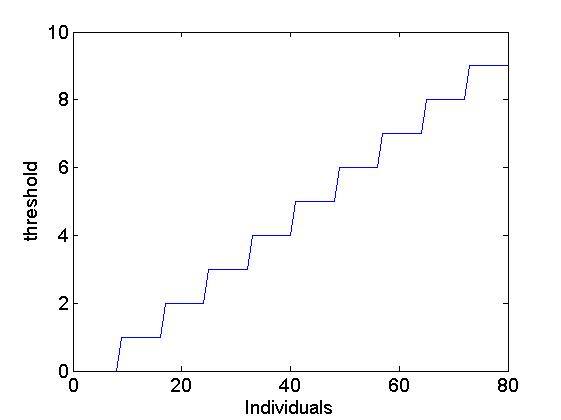
\includegraphics{cascadethresholddistripution.jpg}
\caption{stair like distribution of the thresholds}
\label{cascadethreshold}
\end{figure}

\subsection{Description of the Networks}
\label{subsec:descriptionofnetwork}
As mentioned in section \ref{sec:introAndMotivation} we want to simulate the spread of opinions on a small world network. To have a comparison we also simulated the change of opinions on a random graph. Small world networks and random graphs also have a close connection as figure \ref{influencerewiringprob} shows. In this figure we visualized the Watts and Strogatz model for different rewiring probabilities. If the rewiring probability variies from 0 to 1 a regular graph passes over into a small world network and then into an random graph. In the following we are going to describe the properties of the two network types used in our model.

\begin{figure}
\centering
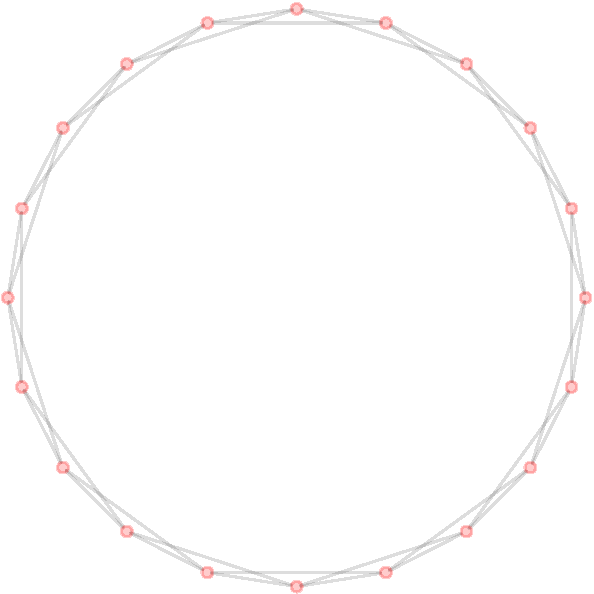
\includegraphics[width= .2 \textwidth]{Influencealphaonnetwork/networkbeta00-crop}
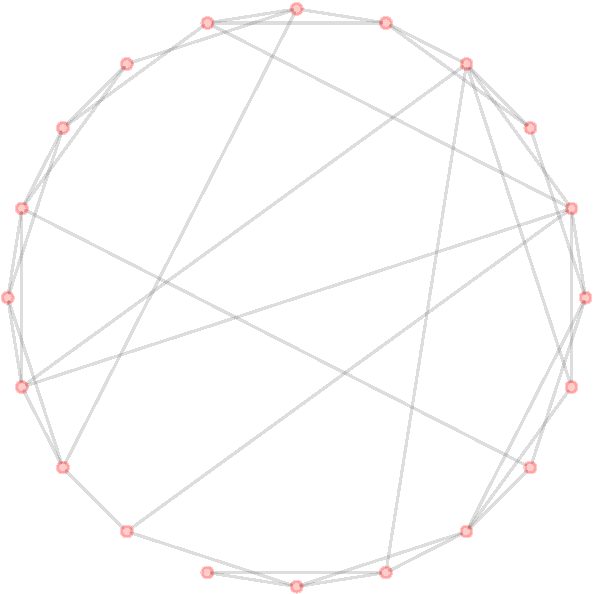
\includegraphics[width= .2 \textwidth]{Influencealphaonnetwork/networkbeta03-crop}
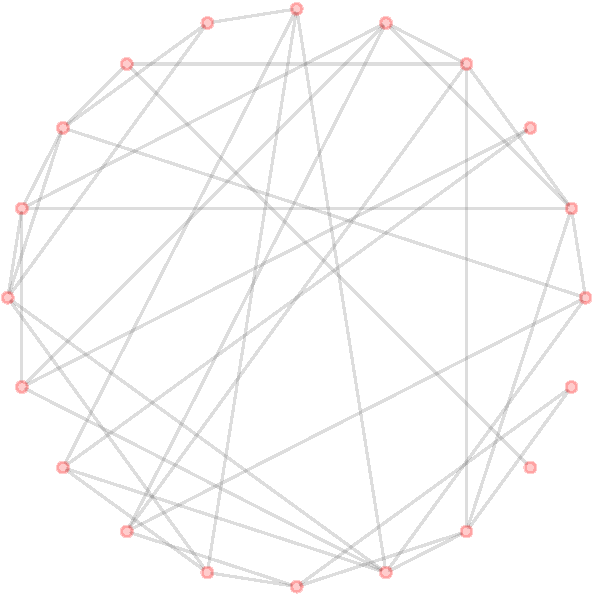
\includegraphics[width= .2 \textwidth]{Influencealphaonnetwork/networkbeta06-crop}
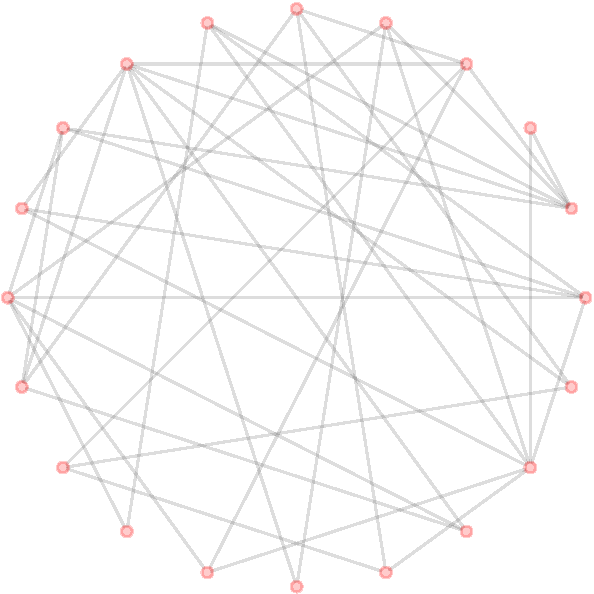
\includegraphics[width= .2 \textwidth]{Influencealphaonnetwork/networkbeta10-crop}
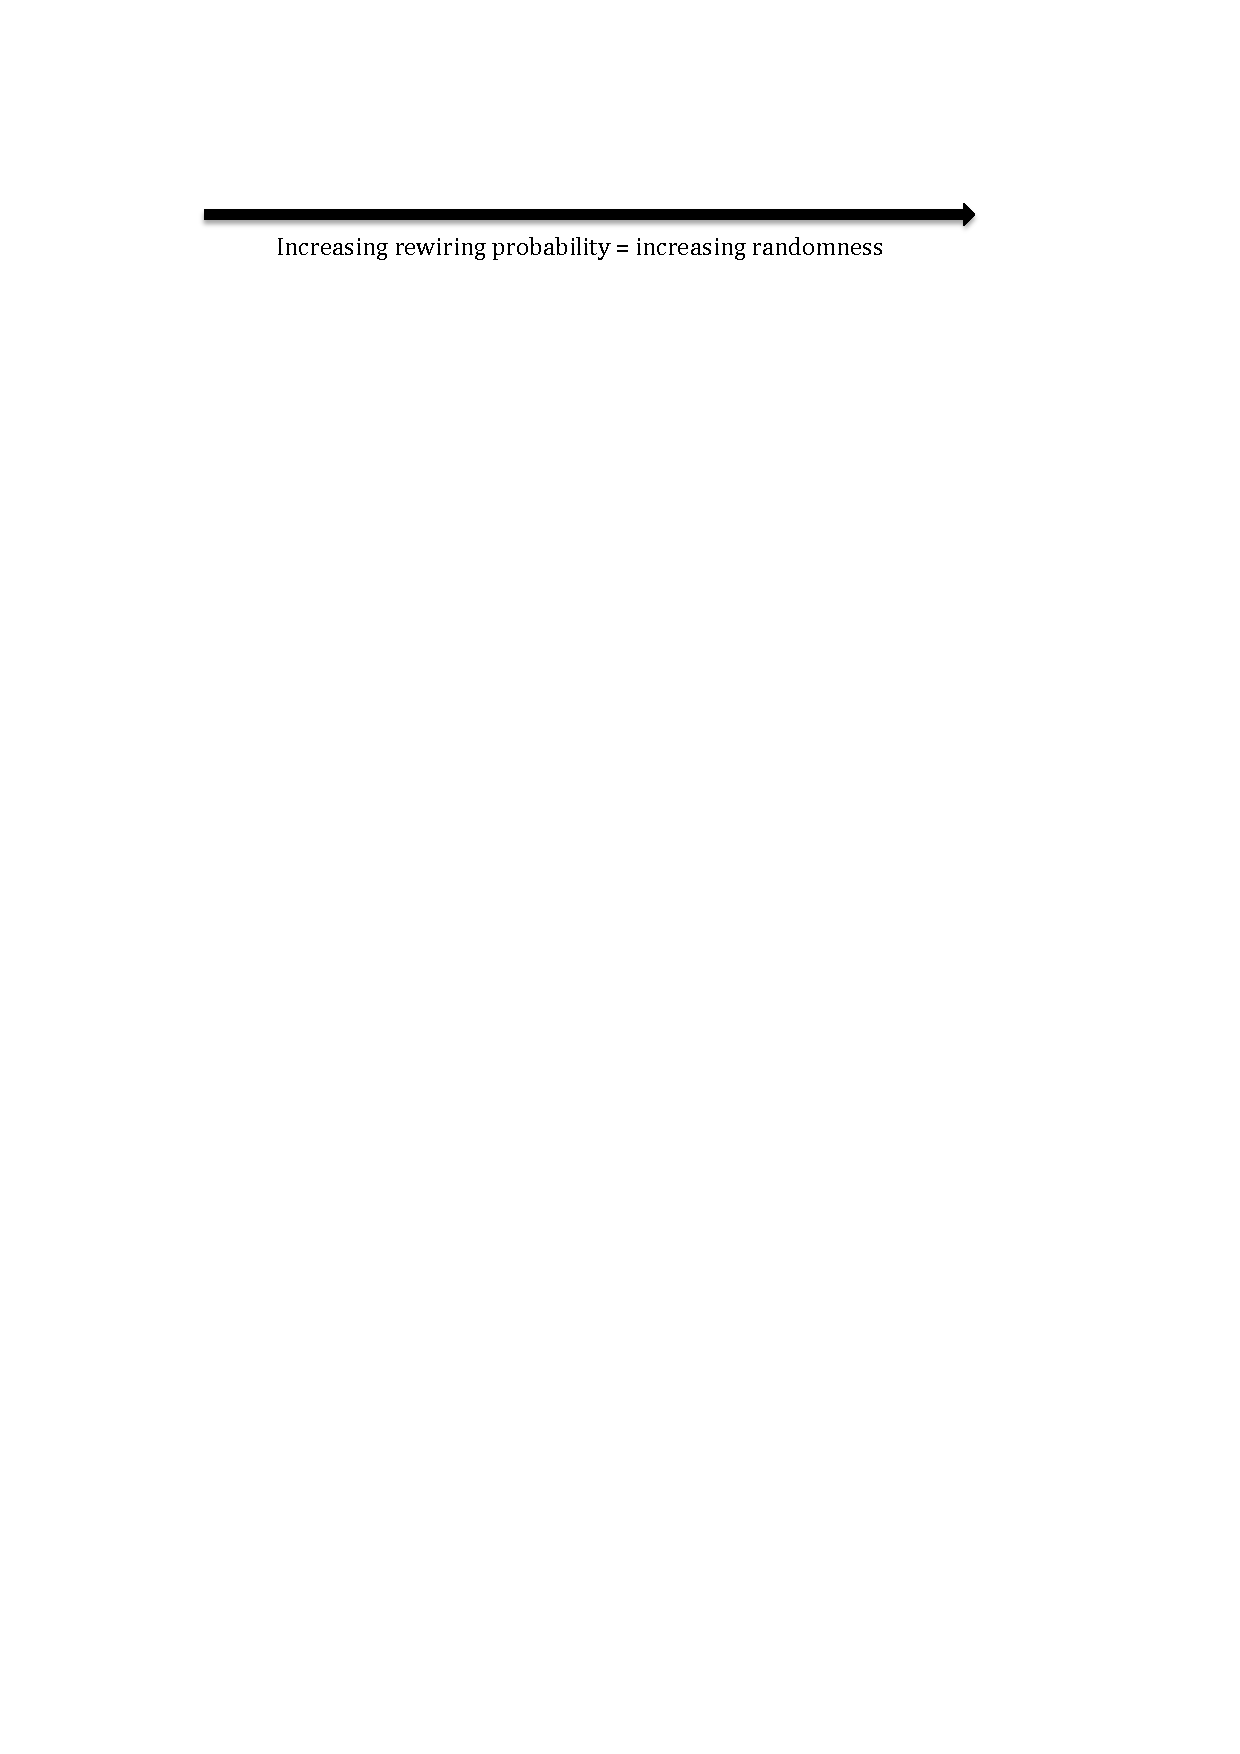
\includegraphics[width= .8 \textwidth]{Influencealphaonnetwork/arrow}
\caption{The influence of the rewiring probability varriing between 0 and 1 on a network with 20 nodes and k = 4 (graphs are generated with the use of the smallworld.m function in the appendix)}
\label{influencerewiringprob}
\end{figure}


\subsubsection{Small World Network}
\label{subsubsec:smallworld}
The most important property of an small world network is that most nodes could be reached from every other by quite a small number of steps. As described in the paper ADDREFERENCE the typical distance L of two random picked nodes is proportional to the log of the total number of nodes.
\begin{equation}
L \propto \log N
\end{equation}
In our model we use the model proposed by Watts and Strogatz. This implements the two main properties of small world networks, which are
\begin{enumerate}
\item small average path length
\item high clustering coefficient
\end{enumerate}
The Watts Strogatz algorithm follows a simple rule. As in figure \ref{influencerewiringprob} the plot on the left shows first there is a regular ring lattice constructed, where every node has exactly for a chosen integer k k neighbours. In a second step every node is taken an rewired with a chosen probability. It is done in a way avoiding loops and duplication \ie connecting a node to itself.\\
A lot of real world examples follow small world type networks. The most famous experiment showing this was done by S. Milgram showing that the average distance between two random persons in the world is five. Other examples that follow the two most important proberties of small world networks are the world wide web, social networks and for example also gene networks. \\
One of the main criticism about small world networks is that they produce unrealistic degree distributions. Many real networks follow the preferential attachement models for example proposed by Barabasi, which give us scale free networks. This means that the produced networks have hubs with a lot of links but also many nodes with just a few links to other nodes. But scale free networks fail to have a high clustering coefficient which also a lot of real world networks have. So neither of the models is perfect.

\subsubsection{Random Graph}
\label{subsubsec:randomgraph}
As the name already says random graphs are generated with some random processes. One of the most important differences of a random graph compared to a small world network is the lack of local clustering. Also the degree distribution is binomial. We used an implementation after a model proposed by $Erd\acute{o}s$ and $R\acute{e}yi$. It could be understood as the limiting case of the Watts Strogatz Algortihm described in section \ref{subsubsec:smallworld} for a rewiring probability of 1. An example is the graph on the right in figure \ref{influencerewiringprob}.
% ---------------------------------*- Latex -*---------------------------------
% Filename: descriptionSolver.tex
% Description: 
% Author: Fabian Wermelinger
% Email: fabianw@student.ethz.ch
% Created: Tue Dec 13 20:40:11 2011 (+0100)
% Version: 
% Last-Updated: Tue Dec 13 22:16:35 2011 (+0100)
%           By: Fabian Wermelinger
%     Update #: 30
% -----------------------------------------------------------------------------
% descriptionSolver.tex starts here
% -----------------------------------------------------------------------------

\subsection{Solving Process}
\label{sec:descriptioSolving}

Once a network has been defined, the relation between the nodes is fully
determined.  If $\mathcal{N}$ is the set of all nodes contained in the network,
then each node $i$ has a set of neighbors $\mathcal{S}_i \subset \mathcal{N}$.
The neighbors $j\in\mathcal{S}_i$ of node $i$ may be \emph{direct} or
\emph{indirect} neighbors.  A direct neighbor $j$ is one that is linked
adjacent to node $i$, where an indirect neighbor node is one that is a neighbor
of a neighbor in a successive fashion.  Each node is characterized by two main
features, \ie, a state and a threshold.
\begin{definition}
  The state of a node is a binary variable.  The value $0$ means that the state
  for a situation is \emph{pro}, whereas the value $1$ is \emph{contra} the
  situation.  The state is subject to change.
\end{definition}
\begin{definition}
  The threshold of a node is a numeric value on the interval $[0,1]$.  A
  threshold of $0$ means that the node will remain in its state no matter what
  the external influences are.  A threshold of $1$ acts opposite.  That is, a
  node with a threshold of $1$ will \emph{always} change its state from pro to
  contra, no matter what the external influences are.  If it already was in
  contra state, it will remain in that state.  Hence, a node with a threshold
  of $1$ acts as a ``seed'' node to initiate some event.  The threshold is a
  constant.
\end{definition}

With the above definitions, the solving process is as follows:
\begin{enumerate}
\item Loop over time
\item Generate a sequential update list
\item Loop over the sequential update list
\item Calculate the neighbor state residual and compare it with the threshold
  of the actual node
\item If the condition applies, update the state of the node
\end{enumerate}

\subsubsection{The Neighbor State Residual}
\label{sec:nbrStateRes}

The neighbor state residual is a scalar which is a measure of an overall state
for all neighbor nodes $j\in\mathcal{S}_i$.  It is used to decide whether a
nodal state is changed by comparing it with the nodal threshold.  If there are
$n$ elements in $\mathcal{S}_i$, then let $\bm{r}_i\in A^n$ be a vector of
dimension $n$, where its elements $r_j$ hold the state of each node
$j\in\mathcal{S}_i$.  The set $A$ holds the two elements $0$ and $1$, which
represent the state.  The neighbor state residual, $\rho_i$, is then defined to
be the Euclidean norm of $\bm{r}_i$, \ie,
\begin{align}
  \label{eq:nbrStateRes}
  \rho_i &= \norm{\bm{r}_i}
\end{align}

So if $\rho_i$ is greater or equal to the threshold of node $i$, then the state
will be forced to contra, \ie, to the value $1$.  The calculation then proceeds
for all nodes in the sequential update list before the next time step is
processed.

%%% Local Variables: 
%%% mode: latex
%%% TeX-master: "master"
%%% End:

% -----------------------------------------------------------------------------
% descriptionSolver.tex ends here
% -----------------------------------------------------------------------------



%%% Local Variables: 
%%% mode: latex
%%% TeX-master: "master"
%%% End: 

\newpage
% ---------------------------------*- Latex -*---------------------------------
% Filename: implementation.tex
% Description: 
% Author: Fabian Wermelinger
% Email: fabianw@student.ethz.ch
% Created: Mon Dec 12 19:08:07 2011 (+0100)
% Version: 
% Last-Updated: Tue Dec 13 22:32:56 2011 (+0100)
%           By: Fabian Wermelinger
%     Update #: 4
% -----------------------------------------------------------------------------
% implementation.tex starts here
% -----------------------------------------------------------------------------

\section{Implementation in \matlab}
\label{sec:implementationMatlab}

The implementation in \matlab is mainly based on functions, which are
sequentially called in a main script file.  All the model parameter are defined
in a single structure, which is passed to all the called functions.  The
parameter and their meaning are also declared in the main script file.  The
main script can be found in Appendix~\ref{sec:main.m}.

\subsection{Implementation of the networks}
\label{sec:implementationofnetworks}

The full code of the network generating functions can be found in
Appendix~\ref{sec:smallworld.m} and Appendix~\ref{sec:randomnetwork}. This section describes shortly the implementation of Section~\ref{sec:descriptionofnetwork} in \matlab code. \\

We used two different implementations for the small world network and the random graph althoug the random graph is just a limiting case in the Watts and Strogatz Model. The Small world model has three input parameters: the total number of nodes, the mean degree and the rewiring probability. The output of the implementation is a sparse symmetric adjacency matrix representing the network graph. We used the format sparse to save memory. The implementation first constructs an regular lattice, where each node has in total the given mean degree. In a second step in two nested for loops we iterate over all nodes exploiting the symmetry and rewire the loops with the specified rewiring propability. As mentioned the output needs to be symmetric which is after the rewiring not the case but now we can make use of the symmetry in order to get the full symmetric adjacency matrix.\\

The random graph is an implementation of the $Erd\acute{o}s$ and $R\acute{e}yi$ model. The input are the total number of nodes and the probability that two nodes are connected and the output is again a sparse symmetric adjacency matrix representing the generated network graph. In the implementation is first the number of non-zero values in every row for a adjacency matrix just containing 0 and 1 generated. In a second step this number is for every row distributed with a binomially distribution with two specified parameters - the total number of nodes and the probability that two nodes are connected. At the end is again made use of the symmetry of the network adjacency matrix. \\

In both implementations we have a big for loop over the network in order to construct the three sub-networks that have some links inbetween.\\

The plots of the networks were done using the igraph library in R. The layout used the in this package implemented Fruchterman and Reingold algorithm, which is a force-based algorithm.
%------------ Latex -----------
%describes the implementation and function of agents.m

\subsection{Implementation of the Agents function}
\label{sec:ImplementAgents }

The complete \matlab code can be found in Appendix ~\ref{sec:agents.m}. The agents function fulfils two purposes. The first is to set end determine the properties every single node(agent) in the network has. As second it acts as interface between the generation of the network and the solver. 

The function consists of a for loop that iterates through all nodes of the network and generates a list containing all the agents, with there properties. These properties are the state, the threshold, a list of all the neighbours and which country or cluster the agent is part of. The state tells whether the agent already joint the revolution(1) or not(0), therefore all agents initially get the value 0. The neighbour property is a list of all the agents the particular agent has a connection to in the network. 

The threshold is the percentage of surrounding agents that sill have to have state 0, so the agent doesn't join the opposition. It gets determined by a  uniformly distributed random number between 0 and 1. Dependent on the given parameters a certain percentage can get a fixed threshold. Furthermore a few agents get a threshold of 1. Those are the agent, that start the revolution. How many of these rebels are placed in the network and how fare they are apart depends on the input parameters. 


% ---------------------------------*- Latex -*---------------------------------
% Filename: implementSolver.tex
% Description: 
% Author: Fabian Wermelinger
% Email: fabianw@student.ethz.ch
% Created: Tue Dec 13 22:16:47 2011 (+0100)
% Version: 
% Last-Updated: Thu Dec 15 21:13:07 2011 (+0100)
%           By: Fabian Wermelinger
%     Update #: 24
% -----------------------------------------------------------------------------
% implementSolver.tex starts here
% -----------------------------------------------------------------------------

\subsection{Implementation of the Solver Function}
\label{sec:implementSolver}

The full code of the solver function can be found in
Appendix~\ref{sec:solverSIRv3.m}.  This section describes the implementation of
Section~\ref{sec:descriptioSolving} in \matlab code.  Additionally, the actual
solver implemented in \matlab also supports a variant of a SIR (Susceptible
Infected Recovered) model for a cellular automaton.

The solver consists mainly of two nested \textsl{for}-loops, where the outer
loop is over a time vector and the inner loop is over a sequential list of
agents, which are to be updated in the active time-step.  In each of these
loops a call to a subroutine may be executed.  Since the subroutines are solver
specific functions, they are appended at the bottom of the solver function.
Therefore, they are only visible to the solver.  The subroutines are
sufficiently commented in the code and will not be discussed here in more
detail.  However, in order to aid the understanding of how the solver works in
general, the statements in the nested loops need further explanation.

The main algorithm starts at line~33 and ends on line~75 in the source code
found in Appendix~\ref{sec:solverSIRv3.m}.  The very first thing that is done
in every time-step is the calculation of the individual cluster residuals, as
well as the global residual for the whole network.  If the whole network
consists of only one cluster, the two residuals are the same.  The calculated
residuals provide a measure of the development of the social behavior over
time.  If it is close to zero, the majority of people are content with the
current situation.  If it is close to one, the opposite is true.  On line~39
the sequential agent update list is calculated.  It is a uniformly distributed
list of random agent indices that get update in the current time-step.  The
list is of random length (also uniformly distributed) but at most
\texttt{maxUpdatedAgents} long.  The constant \texttt{maxUpdatedAgents} is
calculated on line~26 and is some percentage (defined in the parameter
structure) of $\mathcal{N}$, thus, if the set $\mathcal{U}$ contains the
sequential update list of the current time-step, then
$\mathcal{U}\subseteq\mathcal{N}$.

On line~40, a number of noisy agents is calculated in the same way as it is
descried above for the \texttt{maxUpdatedAgents} constant.  The only difference
is that \texttt{nNoize} is a percentage of the set $\mathcal{U}$.  The
\textsl{if}-block from line~42--51 then adds the noize and removes the noisy
agents from the sequential update list.  The update algorithm starts with the
\textsl{for}-loop on line~53.  The algorithm first checks whether the agent is
subject to update.  That is, if its state is zero and if $\rho_i$ is strong
engough to pass the agents threshold.  Then the infection phase of the SIR
implementation takes effect.  If $\beta = 1$, the infection is not applied at
all.  If all of these tests are true, then the agent's state is updated to
contra (\ie, ``$1$'') on line~59.  Note that $\rho_i$ is computed with a
recursive function in order to allow an arbitrary depth of indirect neighbors.
If \texttt{nbrDepth} is set to unity in the parameter list, then only direct
neighbors are taken into account.

The \textsl{if}-block from line~66 to~69 applies the removal phase of the SIR
implementation.  Note that if $\gamma = 0$, the expression is never true and
the removal phase is ignored.  Therfore, if one sets the parameter $\beta = 1$
and $\gamma = 0$, then the SIR model is turned off.  The last \textsl{if}-block
is a write operation, which generates a \texttt{.csv} file.  The file is simply
the list of agents with contra state at the current time-step.  We have used
this file to generate visualizations of time dependent developments in the
network.  We have used R\footnote{R is a collection of software packages for
  statistical computing and graphic generation.  See
  \url{http://www.r-project.org/} for more information.} to generate the
network plots.

\subsubsection{Limitations}
\label{sec:solverLimitations}

The current implementation of the solver function is limited by means that it
only allows state updates in one direction.  That is, an agent's state can only
be changed from pro to contra.  For further development, one may consider to
allow the reverse as well.  However, this implies that if the initial agents
all have a pro state and at least one agent acts as a seed, then noize must be
added in order to allow an agent to change its state in the reverse direction.

The current implementation also assumes that each agent knows all of its direct
and indirect neighbors.  Such an assumption is conservative, as it might be
very well true that an agent only knows some of its neighbors, this is
especially true for the indirect neighbors.  Hence, an additional parameter
could be introduced that defines such behavior.  This would have immediate
effect on $\rho_i$ and eventually influences the decision making of the agent.
Also, note that if the number of indirect neighbors is increased (by increasing
the \texttt{nbrDepth} parameter), the computation time of the solver is also
increased (depending on the network, it may increase drastically).

%%% Local Variables: 
%%% mode: latex
%%% TeX-master: "master"
%%% End:

% -----------------------------------------------------------------------------
% implementSolver.tex ends here
% -----------------------------------------------------------------------------



%%% Local Variables: 
%%% mode: latex
%%% TeX-master: "master"
%%% End: 

% -----------------------------------------------------------------------------
% implementation.tex ends here
% -----------------------------------------------------------------------------

\newpage
\section{Discussion of Results}
\label{sec:discussionofresults}

\subsection{Influence of some parameters in our model}
\subsubsection{Influence of \texttt{noize}}
\label{sec:influencenoize}
As figure \ref{influencenoize} shows, the noize could have quite an influence on the results of the simulation. In our network we have in total 1200 nodes. All the simulations in figure \ref{influencenoize} have the same \texttt{maxUpdate}=0.02. This means that in every time step 24 agents get updated. If the noize is now for example 0.01 only 0.24 agents choose randomly their state. In the case of a noize of 0.1 get 2.4 agents every time step a randomly after a uniform distribution chosen mind state. After this "noize update" the concerned agents are removed from the sequential update list so that they could not be updated twice.\\
As figure \ref{influencenoize} now shows and explained above a noize of 0.01 does not really change the results of the simulation as it has nearly no influence. But as the series of five plots on the right in figure \ref{influencenoize} shows a noize of 10 $\%$ does have quite a big influence on the results of the simulation. Before this big noize the riots where not really starting in the networks now they spread quickly.\\
Compared to reality we think that the noize tends to be close to 0. Who is just completly random changing his mind? It could be that some people change their mind independently from their neighbors and these should be covered by the noize. We think that a noize in reality should be something between 0 and 0.06.

\begin{figure}
\centering
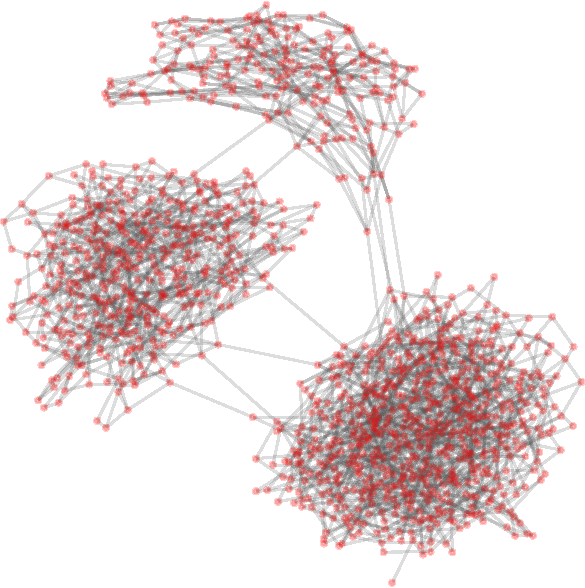
\includegraphics[width=0.25\textwidth]{batchRun__kHalf=2-2-2_maxUpdate=0.02_noize=0_nbrDepth=1/network0-crop.pdf}
\hfill
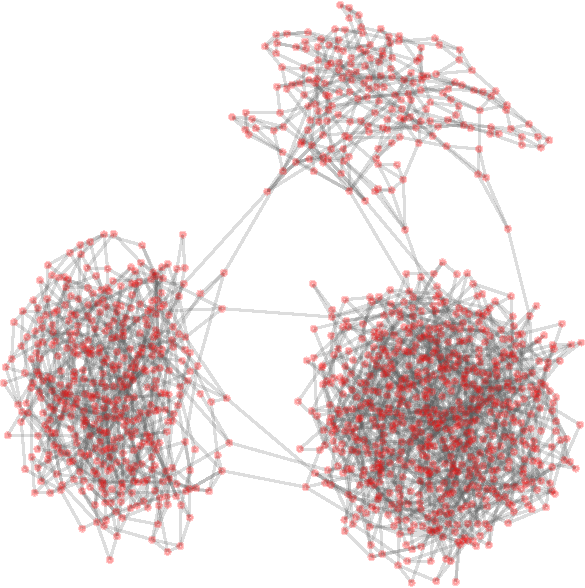
\includegraphics[width=0.25\textwidth]{batchRun__kHalf=2-2-2_maxUpdate=0.02_noize=0.01_nbrDepth=1/network0-crop.pdf}
\hfill
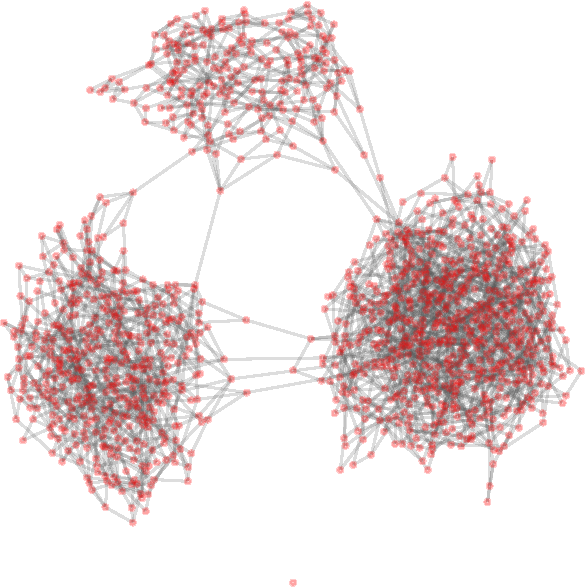
\includegraphics[width=0.25\textwidth]{batchRun__kHalf=2-2-2_maxUpdate=0.02_noize=0.1_nbrDepth=1/network0-crop.pdf}

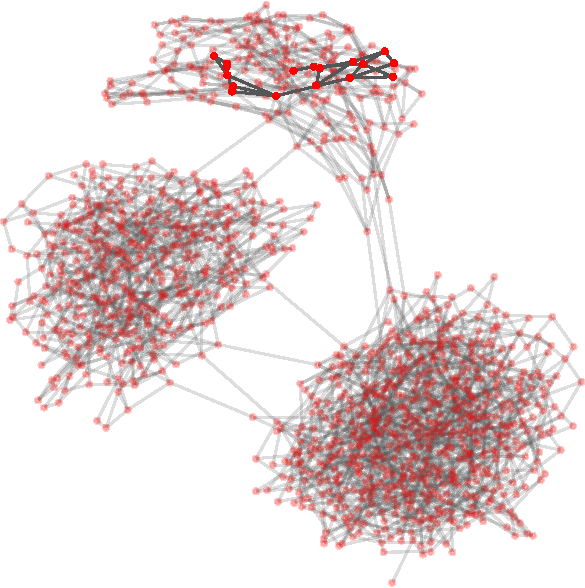
\includegraphics[width=0.25\textwidth]{batchRun__kHalf=2-2-2_maxUpdate=0.02_noize=0_nbrDepth=1/network250-crop.pdf}
\hfill
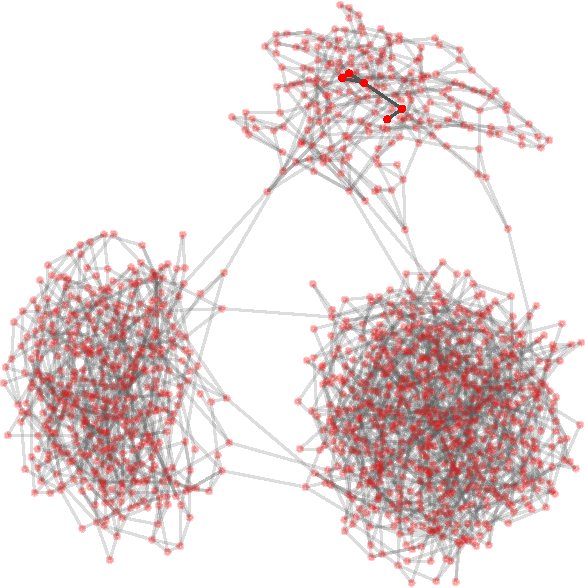
\includegraphics[width=0.25\textwidth]{batchRun__kHalf=2-2-2_maxUpdate=0.02_noize=0.01_nbrDepth=1/network250-crop.pdf}
\hfill
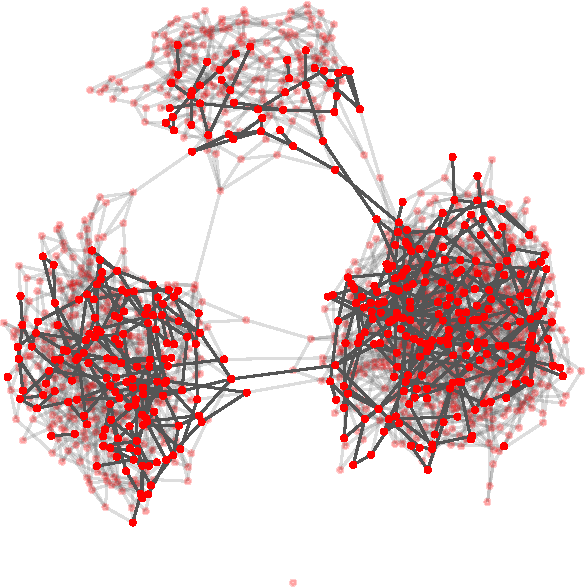
\includegraphics[width=0.25\textwidth]{batchRun__kHalf=2-2-2_maxUpdate=0.02_noize=0.1_nbrDepth=1/network250-crop.pdf}

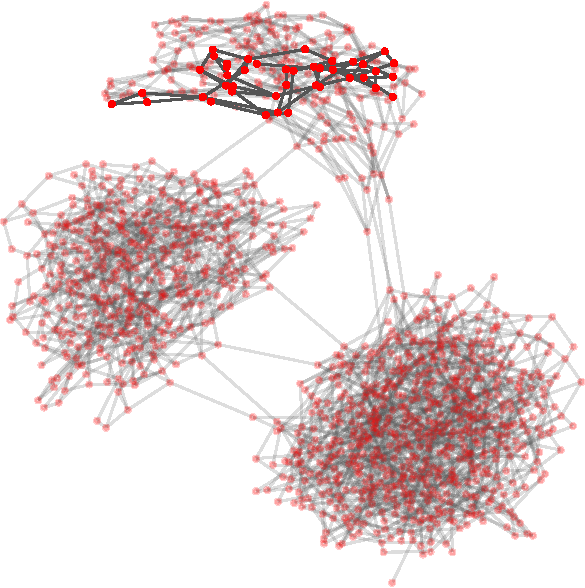
\includegraphics[width=0.25\textwidth]{batchRun__kHalf=2-2-2_maxUpdate=0.02_noize=0_nbrDepth=1/network500-crop.pdf}
\hfill
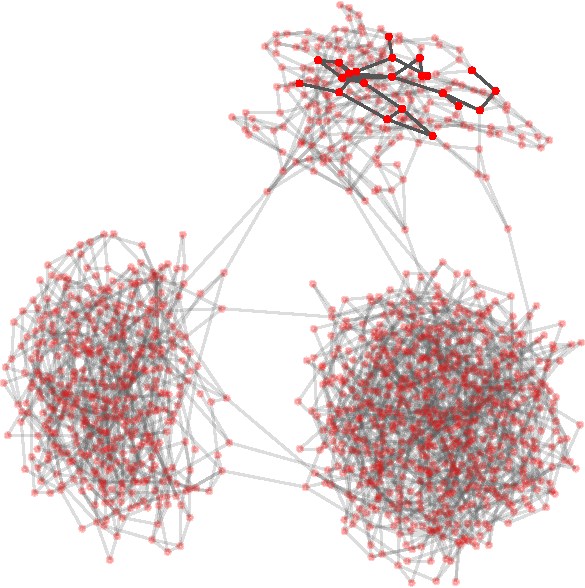
\includegraphics[width=0.25\textwidth]{batchRun__kHalf=2-2-2_maxUpdate=0.02_noize=0.01_nbrDepth=1/network500-crop.pdf}
\hfill
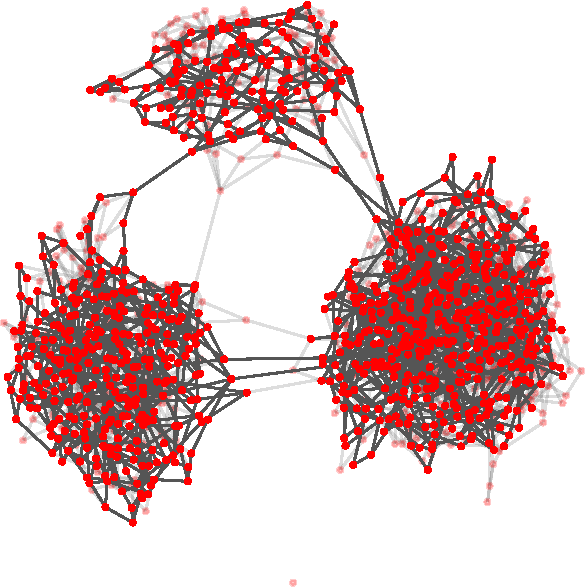
\includegraphics[width=0.25\textwidth]{batchRun__kHalf=2-2-2_maxUpdate=0.02_noize=0.1_nbrDepth=1/network500-crop.pdf}


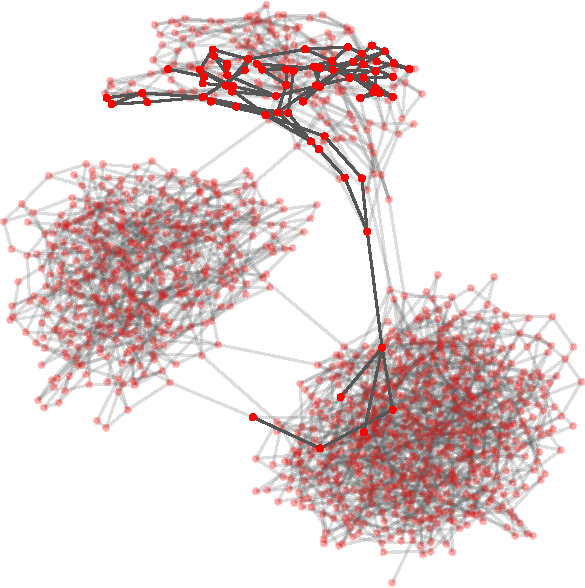
\includegraphics[width=0.25\textwidth]{batchRun__kHalf=2-2-2_maxUpdate=0.02_noize=0_nbrDepth=1/network750-crop.pdf}
\hfill
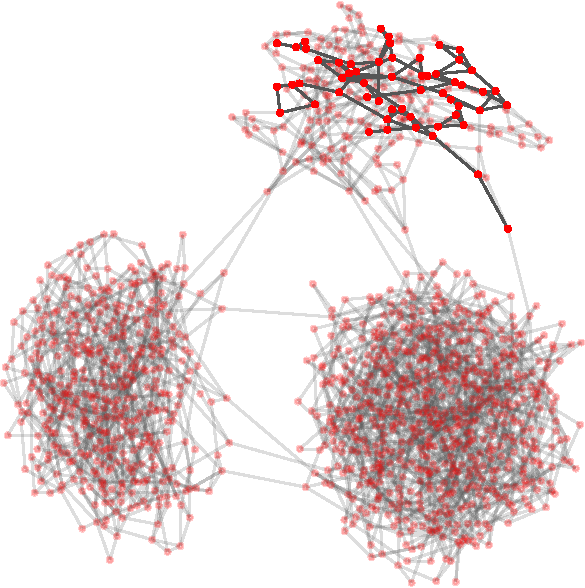
\includegraphics[width=0.25\textwidth]{batchRun__kHalf=2-2-2_maxUpdate=0.02_noize=0.01_nbrDepth=1/network750-crop.pdf}
\hfill
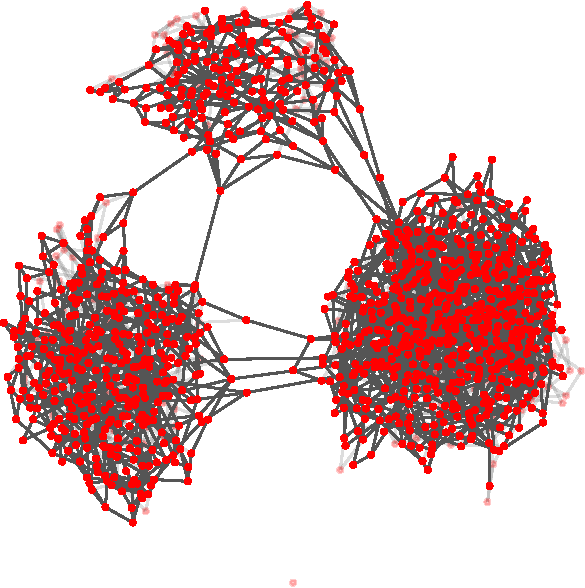
\includegraphics[width=0.25\textwidth]{batchRun__kHalf=2-2-2_maxUpdate=0.02_noize=0.1_nbrDepth=1/network750-crop.pdf}

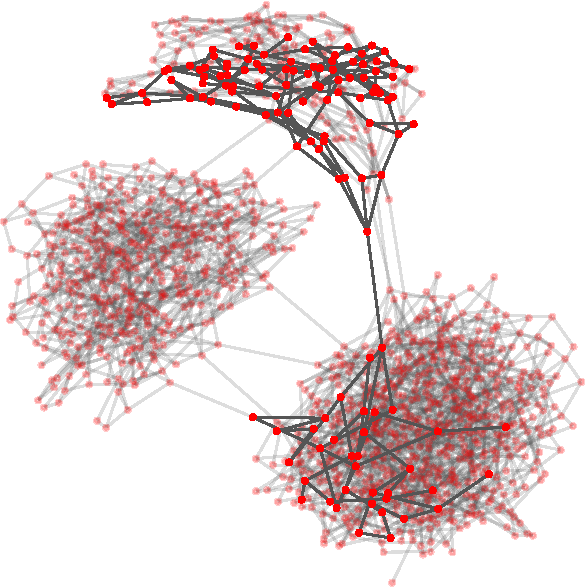
\includegraphics[width=0.25\textwidth]{batchRun__kHalf=2-2-2_maxUpdate=0.02_noize=0_nbrDepth=1/network1000-crop.pdf}
\hfill
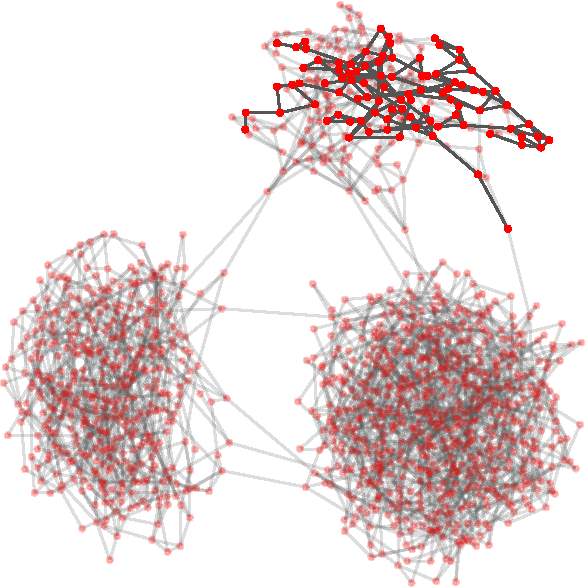
\includegraphics[width=0.25\textwidth]{batchRun__kHalf=2-2-2_maxUpdate=0.02_noize=0.01_nbrDepth=1/network1000-crop.pdf}
\hfill
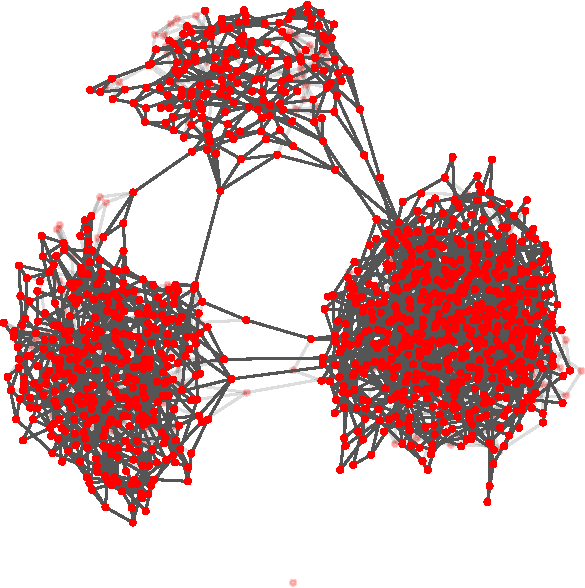
\includegraphics[width=0.25\textwidth]{batchRun__kHalf=2-2-2_maxUpdate=0.02_noize=0.1_nbrDepth=1/network1000-crop.pdf}

\caption{The influence of the noize for the three cases with on the left noize = 0, in the middle 0.01 and on the right 0.1. From top to bottom are the different time steps with the beginning and then increasing in 250 time steps till a 100 time steps.}
\label{influencenoize}
\end{figure}

\subsubsection{Influence of \texttt{maxAgentupdate}}
\label{sec:maxAgentUpdate}



\subsubsection{Influence of \texttt{nbrDepth} = Neighbor Depth}
\label{sec:nbrDepth}

\subsection{Influence of the network type}
\label{sec:influencenetworktype}

\subsection{Comparison to reality}
\label{sec:comparisontoreal}
\newpage
% ---------------------------------*- Latex -*---------------------------------
% Filename: conclusion.tex
% Description: 
% Author: Fabian Wermelinger
% Email: fabianw@student.ethz.ch
% Created: Thu Dec 15 20:23:54 2011 (+0100)
% Version: 
% Last-Updated: Thu Dec 15 20:24:40 2011 (+0100)
%           By: Fabian Wermelinger
%     Update #: 2
% -----------------------------------------------------------------------------
% conclusion.tex starts here
% -----------------------------------------------------------------------------

\section{Conclusion}
\label{sec:conclusion}

All in all our simulations showed some interesting phenomena and sensitivities to different parameters which we are going to summerize in the following. Through the project some interesting new questions arised while others could not be sufficiently be answered. \\
As described in the previous sections the type of the network did not had a to big influence on the results of our simulation. Perhaps were these quite similar results for the different network types a result of the well connected networks we used for most of our simulations. The biggest difference about the random graph and small world network that our simulations showed was that for a random graph the spread of opinions across different clusters was not as predictable as for small world networks. This could be a result that not all the nodes of a random graph have such a short connection as in a small world network. Overall our simulations showed for different parameters that the diffusion of opinions is in small world networks in principal better. \\
Section~\ref{sec:comparisontoreal} showed that there is a relation of the model implemented in \matlab to a real world event.  In order to perform more event specific simulations, parameter sets determined from data of the particular event must be provided.  In general we conclude that the experiment and the model behave closer to each other if the elements in $\mathcal{N}$ and $\mathcal{S}_i$ \emph{increase}.  However, the number of elements in $\mathcal{S}_i$ must still be significantly less than the number of elements in $\mathcal{N}$. \\


%%% Local Variables: 
%%% mode: latex
%%% TeX-master: "master"
%%% End: 

% -----------------------------------------------------------------------------
% conclusion.tex ends here
% -----------------------------------------------------------------------------


\newpage
%BibTeX
\renewcommand{\bibname}{\bibtitle}
\bibliographystyle{siam}
%\addcontentsline{toc}{section}{References}
\bibliography{projectLib}

\newpage

%Appendix
\appendix

\fvset{fontsize=\small, frame=lines,%
  numbers=left, numbersep=3pt, fontshape=sl}
% ---------------------------------*- Latex -*---------------------------------
% Filename: codeMain.tex
% Description: 
% Author: Fabian Wermelinger
% Email: fabianw@student.ethz.ch
% Created: Tue Dec 13 22:26:11 2011 (+0100)
% Version: 
% Last-Updated: Tue Dec 13 22:27:08 2011 (+0100)
%           By: Fabian Wermelinger
%     Update #: 2
% -----------------------------------------------------------------------------
% codeMain.tex starts here
% -----------------------------------------------------------------------------

\section{\texttt{main.m}}
\label{sec:main.m}

\VerbatimInput{../src/main/main.m}


%%% Local Variables: 
%%% mode: latex
%%% TeX-master: "master"
%%% End: 

% -----------------------------------------------------------------------------
% codeMain.tex ends here
% -----------------------------------------------------------------------------
 
\newpage
\section{\texttt{smallworld.m}}
\label{sec:smallworld.m}
The main part of this code was taken from \cite{BruggerSchwirzer2011}.
\VerbatimInput{../src/func/smallworld.m}
\newpage
\section{\texttt{randomgraph.m}}
\label{sec:randomnetwork}

The main part of this code was taken from \cite{BruggerSchwirzer2011}.
\VerbatimInput{../src/func/randomgraph.m}
\newpage


\section{\texttt{Agents.m}}
\label{sec:agents.m}

\VerbatimInput{../src/func/agents.m}


%%% Local Variables: 
%%% mode: latex
%%% TeX-master: "master"
%%% End: 

\newpage
% ---------------------------------*- Latex -*---------------------------------
% Filename: codeSolver.tex
% Description: 
% Author: Fabian Wermelinger
% Email: fabianw@student.ethz.ch
% Created: Mon Dec 12 19:26:08 2011 (+0100)
% Version: 
% Last-Updated: Mon Dec 12 19:35:27 2011 (+0100)
%           By: Fabian Wermelinger
%     Update #: 3
% -----------------------------------------------------------------------------
% codeSolver.tex starts here
% -----------------------------------------------------------------------------

\section{\texttt{solverSIRv3.m}}
\label{sec:solverSIRv3.m}

\VerbatimInput{../src/func/solverSIRv3.m}


%%% Local Variables: 
%%% mode: latex
%%% TeX-master: "master"
%%% End: 

% -----------------------------------------------------------------------------
% codeSolver.tex ends here
% -----------------------------------------------------------------------------


%Backmatter
%------------------------------------------------------------------------------

%Nomenclature
% \markboth{\nomname}{\nomname}
% \printnomenclature

%------------------------------------------------------------------------------
\end{document}
%------------------------------------------------------------------------------

%%% Local Variables: 
%%% mode: latex
%%% TeX-master: t
%%% End: 

%% ----------------------------------------------------------------------------
%%% master.tex ends here
%% ----------------------------------------------------------------------------
